% This is samplepaper.tex, a sample chapter demonstrating the
% LLNCS macro package for Springer Computer Science proceedings;
% Version 2.20 of 2017/10/04
%
\documentclass[runningheads]{llncs}
%
\usepackage{graphicx}
% Used for displaying a sample figure. If possible, figure files should
% be included in EPS format.
%
% If you use the hyperref package, please uncomment the following line
% to display URLs in blue roman font according to Springer's eBook style:
% \renewcommand\UrlFont{\color{blue}\rmfamily}

% Default fixed font does not support bold face
\DeclareFixedFont{\ttb}{T1}{txtt}{bx}{n}{12} % for bold
\DeclareFixedFont{\ttm}{T1}{txtt}{m}{n}{12}  % for normal

% Custom colors
\usepackage{color}
\definecolor{deepblue}{rgb}{0,0,0.5}
\definecolor{deepred}{rgb}{0.6,0,0}
\definecolor{lessdeepred}{rgb}{0.3,0,0}
\definecolor{deepgreen}{rgb}{0,0.5,0}

\usepackage{listings}

% Python style for highlighting
\newcommand\pythonstyle{\lstset{
language=Python,
basicstyle=\ttm,
morekeywords={self},              % Add keywords here
keywordstyle=\ttb\color{deepblue},
emph={MyClass,FeatureExtractor,__init__, None, True},          % Custom highlighting
emphstyle=\ttb\color{deepred},    % Custom highlighting style
stringstyle=\color{deepgreen},
frame=tb,                         % Any extra options here
showstringspaces=false
}}


% Python environment
\lstnewenvironment{python}[1][]
{
\pythonstyle
\lstset{#1}
}
{}

% Python for external files
\newcommand\pythonexternal[2][]{{
\pythonstyle
\lstinputlisting[#1]{#2}}}

% Python for inline
\newcommand\pythoninline[1]{{\pythonstyle\lstinline!#1!}}


\begin{document}
%
\title{Digital Libraries - Document Fingerprints}%\thanks{Supported by organization x.}}
%
%\titlerunning{Abbreviated paper title}
% If the paper title is too long for the running head, you can set
% an abbreviated paper title here
%

\author{Richard Hohensinner\inst{1}\orcidID{MATRIKELNUMMER} \and \\
Inti Gabriel Mendoza Estrada\inst{1}\orcidID{11804156} \and     \\
Jürgen Suntinger-Schrampf\inst{1}\orcidID{00630894}}

\authorrunning{R. Hohensinner et al.}
% First names are abbreviated in the running head.
% If there are more than two authors, 'et al.' is used.
%
\institute{TUGraz, Austria \\ GROUP XXXXXXXX}

\maketitle              % typeset the header of the contribution

\begin{abstract}
The abstract should briefly summarize the contents of the paper in
150--250 words.

\keywords{Document fingerprint  \and Digital libraries \and Visualisation.}
\end{abstract}
%
%
%

\section{Introduction}
As the world enters an era defined by \textit{big data}, more and more information is being actively accrued. This vast amount of data is not immediately available to people. It must now be accessible. What libraries did for physical books, digital libraries are doing for digital data. Challenges begin to appear when you consider that data can come in a vast array of ways (on top of the actual amount of data). When challenges appear, however, their solutions end up, most often than not, incredibly useful. Digital libraries not only let you access texts, papers, books. You are able to access videos, images, 3D models\ldots What makes digital libraries so incredibly useful lies in the fields it comprises: Computer Science, Information Science, and Information Visualisation - to name a few. 

In Computer Science comes something called \textit{Natural Language Processing} (or NLP). NLP is the automatic understanding of text by a computer. Being able to "understand" text is immensely useful. In the field of Digital Libraries, therefore, you can not only access text via keywords or titles but also through what the text actually means and compels.

What if you could search through a text based on the emotions of sentences? What if you could find texts that are easy to read based on sentence length? What if you could find texts to improve your language skills based on sentence complexity? What if you could use NLP to train a Neural Network to guess the genre of a text? This is the motivation that made us develop a tool that is able to create a visual "fingerprint" of a document to compare and contrast entire texts against others simultaneously on top of being able to compare and contrast sections within a given text.



was ist idee


Used data

o Introduction: Search/Exploration problem and user tasks to support o Short related work section with similar systems you know
o Your project solution
Development environment (language, libraries, ...) Implemented functionalities
Description of supported user operations (workflows)
o Application demonstration
Demonstrate the supported user operations by a walkthrough of a hypothetical
user Alice considering the used data
Describe how and where searching and exploring are possible
Describe interesting findings and observations you made when applying your solution to the data
o Discussion of advantages, limitations and future developments to do
           
Digital Libraries 2020/21, Assignment specifications Version: October 30, 2020, 21:45
 o Statement of contributions of team members to the project (design, coding, application, report writing)
o References Hints for the report:
Please use the Springer LNCS Word or LaTeX Template12 for the report Aim for not more than 10 pages + appendix
Make use of images/screenshots for your results, use selected ones in the main text, and more suporting images in the appendix
Make use of diagrams to show system architcute or workflows



\newpage
\section{Development of our Tool}
In this section we divide the three areas of software engineering that were developed in the creation of our tool. 

\subsection{Back-End: Feature Extraction}

Using NLP, we should be able to obtain features from a given text. Features such as word length, sentence length, sentiment of a sentence, etc\ldots We developed the file \texttt{feature\_extraction.py} to take care of just that. We used the programming language \texttt{Python} for this task due to it being incredibly powerful and easy to use in data-related tasks. Furthermore the \texttt{Natural Language Toolkit} library is supported by \texttt{Python}. This tool allows the programmer to use symbolic and statistical natural language processing for the English language.

\subsubsection{Natural Language Toolkit}

The \texttt{Natural Language Toolkit} (or NLTK) library is downloaded and installed into one's \texttt{Python} environment through the following line of code:

\begin{python}
nltk.download()
\end{python}

From the NLTK library we use the following functions:
\begin{itemize}
    \item[--] Sentence Tokenizer: from a text, return a list of the entire text separated per sentence.
    \item[--] Word Tokenizer: from a text, return a list of the entire text separated per word.
    \item[--] Porter Stemmer: from a given word, return the root of it using a Porter Stemmer algorithm.
    \item[--] Stop Words: returns a list of all stop words from the English language (words with no inherent meaning - such as the words "the" and "a".)
    \item[--] Sentiment Intensity Analyser: from a sentence, return a dictionary containing the negative, neutral, positive, and compound values from that sentence.
\end{itemize}

We imported them into our \texttt{Python} file as such:

\begin{python}
from nltk.tokenize import sent_tokenize, \
word_tokenize, TextTilingTokenizer
from nltk.stem import PorterStemmer
from nltk.corpus import stopwords
from nltk.sentiment.vader import \ 
SentimentIntensityAnalyzer
\end{python}

Our \pythoninline{class FeatureExtractor} is defined as follows:
\begin{python}
class FeatureExtractor(object):
	exclude_stop_words = 	True
	stem_words = 		True
	filter_integers = 	True
	exclude_duplicates =	True

	ps = None

	average_word_length_per_sentence =  None
	words_per_sentence =                None
	length_per_sentence =               None
	richness_per_sentence =             None
	richness_per_x_words =              None
	richness_per_sentence_stemmed =     None
	richness_per_x_words_stemmed =      None
	sentiment_per_sentence =            None
	digit_count_per_sentence =          None

	def __init__(self, exclude_stop_words \
	= False, stem_words = False, \
	filter_integers = False, \
	exclude_duplicates = False):
		self.exclude_stop_words = \
		exclude_stop_words
		self.stem_words = \
		stem_words
		self.filter_integers = \
		filter_integers
		self.exclude_duplicates = \
		exclude_duplicates

		self.ps = PorterStemmer()
\end{python}

\subsection{Back-End: Server}

\subsection{Front-End}






%
%\section{First Section}
%\subsection{A Subsection Sample}
%Please note that the first paragraph of a section or subsection is
%not indented. The first paragraph that follows a table, figure,
%equation etc. does not need an indent, either.
%
%Subsequent paragraphs, however, are indented.
%
%\subsubsection{Sample Heading (Third Level)} Only two levels of
%headings should be numbered. Lower level headings remain unnumbered;
%they are formatted as run-in headings.
%
%\paragraph{Sample Heading (Fourth Level)}
%The contribution should contain no more than four levels of
%headings. Table~\ref{tab1} gives a summary of all heading levels.
%
%\begin{table}
%\caption{Table captions should be placed above the
%tables.}\label{tab1}
%\begin{tabular}{|l|l|l|}
%\hline
%Heading level &  Example & Font size and style\\
%\hline
%Title (centered) &  {\Large\bfseries Lecture Notes} & 14 point, bold\\
%1st-level heading &  {\large\bfseries 1 Introduction} & 12 point, bold\\
%2nd-level heading & {\bfseries 2.1 Printing Area} & 10 point, bold\\
%3rd-level heading & {\bfseries Run-in Heading in Bold.} Text follows & 10 point, bold\\
%4th-level heading & {\itshape Lowest Level Heading.} Text follows & 10 point, italic\\
%\hline
%\end{tabular}
%\end{table}
%
%
%\noindent Displayed equations are centered and set on a separate
%line.
%\begin{equation}
%x + y = z
%\end{equation}
%Please try to avoid rasterized images for line-art diagrams and
%schemas. Whenever possible, use vector graphics instead (see
%Fig.~\ref{fig1}).
%
%\begin{figure}
%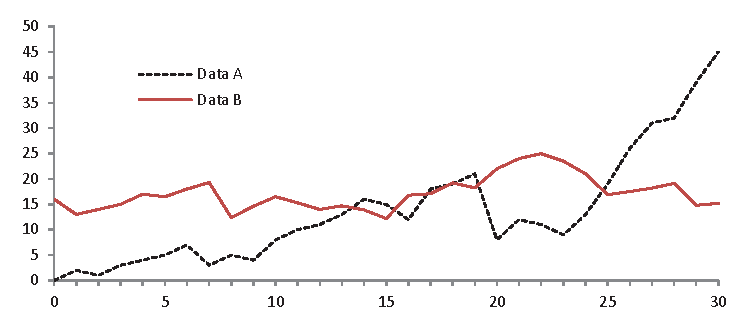
\includegraphics[width=\textwidth]{fig1.eps}
%\caption{A figure caption is always placed below the illustration.
%Please note that short captions are centered, while long ones are
%justified by the macro package automatically.} \label{fig1}
%\end{figure}
%
%\begin{theorem}
%This is a sample theorem. The run-in heading is set in bold, while
%the following text appears in italics. Definitions, lemmas,
%propositions, and corollaries are styled the same way.
%\end{theorem}
%%
%% the environments 'definition', 'lemma', 'proposition', 'corollary',
%% 'remark', and 'example' are defined in the LLNCS documentclass as well.
%%
%\begin{proof}
%Proofs, examples, and remarks have the initial word in italics,
%while the following text appears in normal font.
%\end{proof}
%For citations of references, we prefer the use of square brackets
%and consecutive numbers. Citations using labels or the author/year
%convention are also acceptable. The following bibliography provides
%a sample reference list with entries for journal
%articles~\cite{ref_article1}, an LNCS chapter~\cite{ref_lncs1}, a
%book~\cite{ref_book1}, proceedings without editors~\cite{ref_proc1},
%and a homepage~\cite{ref_url1}. Multiple citations are grouped
%\cite{ref_article1,ref_lncs1,ref_book1},
%\cite{ref_article1,ref_book1,ref_proc1,ref_url1}.
%%
%% ---- Bibliography ----
%%
%% BibTeX users should specify bibliography style 'splncs04'.
%% References will then be sorted and formatted in the correct style.
%%
%% \bibliographystyle{splncs04}
%% \bibliography{mybibliography}
%%
%\begin{thebibliography}{8}
%\bibitem{ref_article1}
%5Author, F.: Article title. Journal \textbf{2}(5), 99--110 (2016)
%
%\bibitem{ref_lncs1}
%Author, F., Author, S.: Title of a proceedings paper. In: Editor,
%F., Editor, S. (eds.) CONFERENCE 2016, LNCS, vol. 9999, pp. 1--13.
%Springer, Heidelberg (2016). \doi{10.10007/1234567890}
%
%\bibitem{ref_book1}
%Author, F., Author, S., Author, T.: Book title. 2nd edn. Publisher,
%Location (1999)
%
%\bibitem{ref_proc1}
%Author, A.-B.: Contribution title. In: 9th International Proceedings
%on Proceedings, pp. 1--2. Publisher, Location (2010)
%
%\bibitem{ref_url1}
%LNCS Homepage, \url{http://www.springer.com/lncs}. Last accessed 4
%Oct 2017
%\end{thebibliography}
\end{document}
